\chapter{Marco Teórico}\label{chapter:theory}

\todounsure{Sobre uso de siglas STM/LTM... es necesario usar siempre las siglas???, pues a veces puede ser un poco tedioso leer lo mismo cada vez.}

\todoimprove{Ojo con citas y et al. Normalizar esto. Ver: \url{http://biblioinstruccion.blogspot.com/2010/04/como-utilizar-el-et-al-en-las-citas-y.html}}

En este capítulo se revisan los temas y conceptos teóricos relevantes para el desarrollo del trabajo. Se formaliza la definición de robot doméstico y sus alcances. Se describe la memoria humana, sus categorías, funcionamiento y procesos cerebrales relevantes. Basado en los temas anteriores, se revisa la relación entre robótica y la memoria humana: se describen algunos enfoques existentes y las reglas generales para su implementación.

%% =====================================================================
\section{Robots de servicio domésticos}\label{sec:domestic_robots}
%% =====================================================================
%% =====================================================================
%% =====================================================================
%% =====================================================================

La Federación Internacional de Robótica (IFR) \cite{IFR} define \textit{robot} como:
\begin{quotation}
	``Un mecanismo actuado y programable en dos o más ejes y con un cierto grado de autonomía, que se mueve en su entorno para realizar tareas previstas. En este contexto, autonomía se refiere a la habilidad de realizar tareas previstas, basado en el estado actual y lo sensado, sin intervención humana.''
\end{quotation}

Asimismo, la IFR define un \textit{robot de servicio} como un robot ``que realiza tareas útiles para humanos o equipamiento, excluyendo aplicaciones de automatización industrial''. Así, un robot de servicio debe trabajar en ambientes no controlados y con la autonomía suficiente que le permita llevar a cabo su cometido. Generalmente, la robótica de servicio se enfoca en asistir a los seres humanos en tareas repetitivas y comunes.

Según su área de aplicación, un robot de servicio se clasifica en \textit{de uso personal} o \textit{de uso profesional}. Los primeros son utilizados en ambientes no comerciales y por personas comunes; como por ejemplo, un robot sirviente o una silla de ruedas autónoma. Un robot de servicio profesional se utiliza en ambientes comerciales, usualmente operados por alguien entrenado; un ejemplo son los robots de entrega de paquetes o para cirugía.


Según la recopilación de datos realizada por la IFR durante el 2016, este tipo de robots es utilizado en las siguientes áreas:
\begin{itemize}
	\item Tareas domésticas: De compañía, asistencia, limpieza, cuidado del hogar.
	\item Entretenimiento: Juguetes, comunicación, educación e investigación.
	\item Asistencia a ancianos y discapacitados: Sillas robóticas y robots para cuidar personas.
	\item Transporte.
	\item Seguridad y vigilancia.
	\item Otros que no caen en las categorías anteriores.
\end{itemize}
\bigskip

El foco de este trabajo son los robots de servicio personales, dedicados a tareas domésticas, clasificación a la que en  adelante se referirá como \textit{Robots Domésticos}.

Para entender el alcance del trabajo, en cuanto a qué es lo que se espera del sistema, a continuación se listan algunas capacidades de los robots domésticos. Un robot de compañía y asistencia tiene, pero no se limita a las siguientes tareas:
\begin{itemize}
	\item Interacción amistosa con humanos.
	\item Ayudar a recordar y organizar tareas.
	\item Cooperar con la realización de un procedimiento.
	\item Guiar y seguir a personas.
	\item Recordar información y entidades.
\end{itemize}
\bigskip

Algunas tareas que robots domésticos de tipo mayordomo deben ejecutar son:
\begin{itemize}
	\item Ofrecer comida y bebestibles.
	\item Preparación de comida.\setcounter{tocdepth}{4}
	\item Ordenar y limpiar el hogar.
\end{itemize}
\bigskip


%% =====================================================================

%% =====================================================================

%% =====================================================================

%% =====================================================================

%% =====================================================================

%% =====================================================================

%% =====================================================================

%% =====================================================================

%% =====================================================================
\section{Memoria humana}\label{sec:human_memory}
%% =====================================================================
%% =====================================================================
%% =====================================================================
%% =====================================================================

La memoria es un elemento fundamental para los humanos en su día a día, es parte integral de su existencia. Permite recordar quién, qué, cómo, dónde y cuándo. En términos psicológicos, es la habilidad para codificar, almacenar y luego obtener información sobre eventos pasados, en el cerebro. Los pensamientos son parte de la memoria de corto plazo, mientras que eventos pasados son almacenados en una memoria de largo plazo. Existen muchos estudios en el área de la psicología cognitiva con diversas descripciones y modelos teóricos de cada tipo de memoria \cite{Vijayakumar2014}.

Desde el punto de vista de la información procesada, la memoria es vista como una facultad humana consistente en procesos para el manejo de información. Los 3 componentes principales son:

\begin{itemize}[topsep=0pt]
	\setlength\itemsep{0.2em}
	\item \textbf{Codificación}: En este paso, se adquiere nueva información desde los sentidos humanos. Los datos son convertidos a un formato que pueda ser almacenado en la estructura cerebral correspondiente.
	\item \textbf{Almacenamiento}: Consiste en la creación de registros permanentes de información. Es un proceso pasivo, de continuo procesamiento para clasificar datos nuevos y los ya existentes en el cerebro.
	\item \textbf{Adquisición}: Hace referencia al acceso de datos almacenados. El proceso se realiza en respuesta a una pista, que permita obtener una reconstrucción aproximada de la información, a partir de elementos repartidos en distintas partes del cerebro.
\end{itemize}
%\bigskip

La memoria puede ser dividida en múltiples sistemas de independientes, con funcionalidades bien definidas y sustentados por distintas estructuras cerebrales \cite{pmid-Squire}. La primera diferenciación define dos tipos de memoria: la de corto y la de largo plazo, \textbf{STM (Short-Term Memory)} y \textbf{LTM (Long-Term Memory)}, por sus siglas en inglés \cite{pmid10643472}. En el diagrama de la Figura \ref{img:human_memory} se muestra una separación clásica utilizada en el área de las ciencias cognitivas \cite{Eichenbaum:2008}, explicada en las siguientes subsecciones.

\usetikzlibrary{arrows,shapes,positioning,shadows,trees}
\tikzset{
	basic/.style  = {draw, drop shadow, font=\sffamily, rectangle},
	root/.style   = {basic, rounded corners=2pt, text width=10em, very thick, align=center, fill=gray!5},
	level 1/.style = {sibling distance=20mm},
	level 2/.style = {basic, rounded corners=6pt, thin,align=center, fill=red!10, text width=8em},
	level 3/.style = {basic, rounded corners=2pt, thin, align=center, fill=gray!10, text width=6.5em},
	level 4/.style = {basic, thin, align=left, fill=blue!10, text width=10em}
}

\begin{figure}[!h]
	\centering
	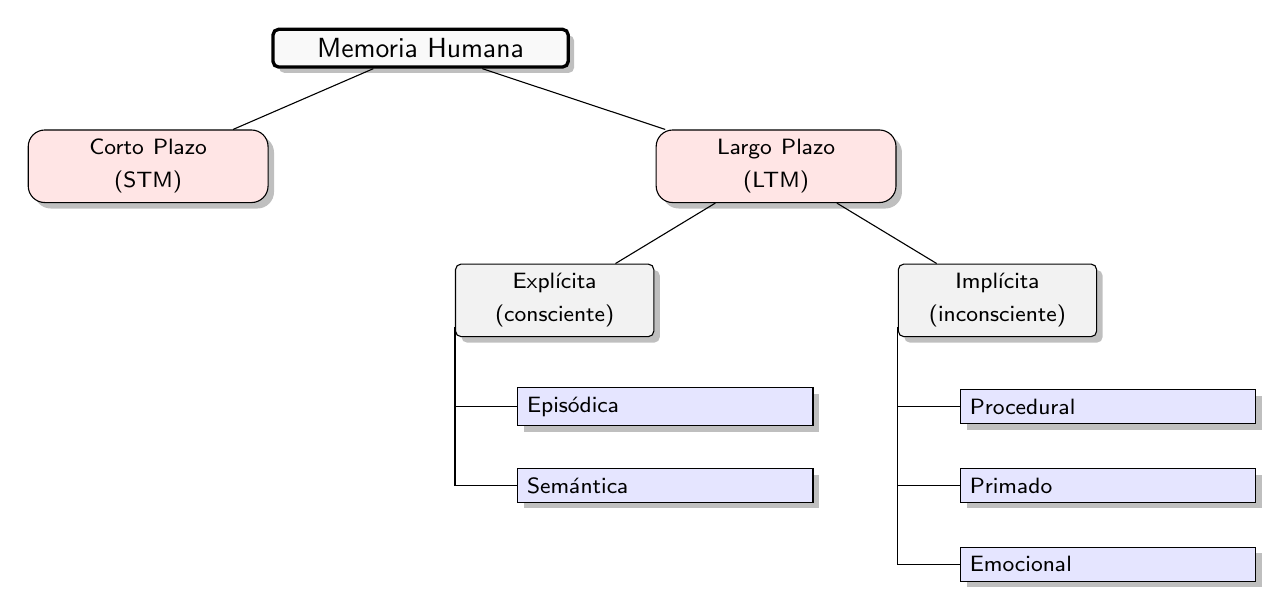
\begin{tikzpicture}[]
	
	\node [root] {Memoria Humana}
	child { node [level 2, xshift=-70pt] (c1) {\footnotesize Corto Plazo\\ (STM) }}
	child { node [level 2, xshift=100pt] (c2) {\footnotesize Largo Plazo\\ (LTM) }};
	
	\begin{scope}[every node/.style={level 3}]
	\node [below of = c2, xshift=-80pt, yshift=-20pt] (c21) {\footnotesize Explícita\\ (consciente)};  
	\node [below of = c2, xshift=80pt, yshift=-20pt] (c22) {\footnotesize Implícita\\ (inconsciente)};
	\end{scope} 
	
	\begin{scope}[every node/.style={level 4}]
	\node [below of = c21, xshift=40pt, yshift=-10pt] (c211) {\footnotesize Episódica};
	\node [below of = c211, xshift=0pt, yshift=0pt] (c212) {\footnotesize Semántica};
	
	\node [below of = c22, xshift=40pt, yshift=-10pt] (c221) {\footnotesize Procedural};
	\node [below of = c221, xshift=0pt, yshift=0pt] (c222) {\footnotesize Primado};
	\node [below of = c222, xshift=0pt, yshift=0pt] (c223) {\footnotesize Emocional};
	\end{scope} 
	
	\draw[-, to path={-- (\tikztotarget)}]
	(c2) edge (c21)
	(c2) edge (c22);
	
	\draw[-, to path={|- (\tikztotarget)}]
	(c21.195) edge (c211.west)
	(c21.195) edge (c212.west);
	
	\draw[-, to path={|- (\tikztotarget)}]
	(c22.195) edge (c221.west)
	(c22.195) edge (c222.west)
	(c22.195) edge (c223.west);
	
	\end{tikzpicture}
	\caption{\small Clasificaciones de la memoria humana. Adaptado de \cite{Vijayakumar2014}.}
	\label{img:human_memory}
\end{figure}



%% =====================================================================
%% =====================================================================
%% =====================================================================
\subsection{Memoria de corto plazo (STM)}
%% =====================================================================
%% =====================================================================
%% =====================================================================


En el ámbito cognitivo, la STM se refiere a la habilidad de estar atento, recopilar información  y memorias, para luego utilizarlas dentro de un corto periodo de tiempo \cite{Eichenbaum:2008}. Es responsable de almacenar información constantemente y de decidir que parte será transferida a la memoria de largo plazo. El término de \textit{Memoria de Trabajo} suele ser utilizado de manera intercambiable con el de STM.

Se caracteriza por manejar información muy detallada, ser de poca capacidad y permitir un rápido acceso a estos datos. Permite recordar rápidamente y con gran detalle experiencias ocurridas hace pocos segundos, pero con dificultad creciente a medida que avanza el tiempo.

Se sustenta principalmente en la corteza prefrontal del cerebro. Algunos estudios han mostrado que las neuronas involucradas son capaces de mantener información relevante de corto plazo, la que es combinada con información sensorial entrante y áreas que manejan la toma de decisiones. 

En los humanos esta área presenta gran activación durante procesos de codificación, acceso y manipulación de memorias.


%% =====================================================================
%% =====================================================================
%% =====================================================================
\subsection{Memoria de largo plazo (LTM)}
%% =====================================================================
%% =====================================================================
%% =====================================================================


La LTM se asocia al almacenamiento permanente de información en el cerebro. Se caracteriza por manejar una gran cantidad de experiencias y entidades, ser menos detallada y proveer un acceso más lento a los recuerdos, respecto a la STM \cite{Eichenbaum:2008}. Cierta información de la STM eventualmente es transferida a la LTM. De acuerdo a la Figura \ref{img:human_memory}, sus dos principales categorías son la \textit{Memoria Implícita} y la \textit{Memoria Explícita}.


\subsubsection{Memoria de largo plazo explícita}
%% =====================================================================

La memoria explícita suele ser denominada \textit{memoria consciente} o \textit{memoria declarativa}, pues maneja conocimientos relacionados a hechos y eventos adquiridos de forma consciente. Según las estructuras cerebrales involucradas, se conforma de la \textit{memoria episódica} y de la \textit{memoria semántica} \cite{Eichenbaum:2008}.

La \textbf{memoria episódica}, por primera vez definida por Tulving \cite{2_tulving}, es de carácter  autobiográfico y almacena detalles de eventos y experiencias pasadas. Permite responder a las preguntas ``Qué sucedió'', ``Dónde ocurrió'' y ``Cuándo ocurrió'' \cite{Deutsch2008}. Particularmente, se utiliza la noción de memoria episódica descrita por Clayton y Russel \cite{CLAYTON20092330}, que incorpora el concepto de perspectiva episódica de los recuerdos. Un humano puede acceder a esta memoria si es capaz de decir: ``recuerdo que''. Este tipo de memoria da al ser humano la sensación de continuidad en el tiempo.

La \textbf{memoria semántica} almacena el conocimiento de hechos, significados, categorías y proposiciones. Un humano puede acceder a esta memoria si es capaz de decir: ``sé que''. Esta memoria se abstrae de perspectiva e información situacional.

Las estructuras cerebrales que soportan la memoria explícita son el hipocampo, encargado de manejar la memoria episódica, junto a la corteza cerebral, en donde se distribuyen los conocimientos de la memoria semántica. En el hipocampo se mantienen conexiones neuronales a los sectores de interés de la corteza, en donde se alojan conocimientos semánticos asociados a cada episodio.

Un ejemplo de uso de memoria episódica es el recuerdo de una graduación escolar, el lugar y la fecha donde ocurrió. La memoria semántica podría responder en que consiste una graduación y describir la ropa que se suele ocupar en ellas.



\subsubsection{Memoria de largo plazo implícita}
%% =====================================================================

La memoria implícita abarca la capacidad de aprender habilidades, hábitos y preferencias, caracterizados por ser mejorados o adquiridos sin una recolección consciente. Así, también suele ser denominada \textit{memoria inconsciente} o \textit{memoria no declarativa}, pues comprende acciones que pueden ser realizadas sin pensar en ellas. Ejemplos de esto, son el andar en bicicleta o tocar un instrumento musical \cite{Eichenbaum:2008}.

Dos de sus componentes son la \textit{memoria procedural} y la \textit{memoria de primado}. La primera ayuda a realizar tareas sin pensar en ellas, es decir, maneja el conocimiento del \textit{Cómo}; Ejemplos de esto son comer y caminar. La memoria de primado hace referencia a la predisposición para recordar hechos o información a la que un sujeto es expuesto con anterioridad; Ejemplos de esto son la facilidad para recordar canciones escuchadas hace poco tiempo, o el uso de palabras e ideas vistas recientemente.

Se ha mostrado que la memoria procedural se sustenta en el cerebelo, mediante la activación de este durante el uso de habilidades motoras.

Un tercer componente de la memoria implícita es la \textbf{memoria emocional} \cite{episodic_philip}. Esta se encarga de dar significado afectivo a ciertos estímulos, que de otra forma serían neutrales. Las estructuras cerebrales involucradas son la amígdala, las áreas corticales y subcorticales. Esta memoria se expresa mediante la activación del hipotálamo, en conjunto al sistema nervioso simpático, generando reacciones emocionales y sentimientos.


\subsection{Plasticidad sináptica y modulación}
%% =====================================================================

Se denomina \textit{consolidación} de memoria al proceso de transición de conocimiento desde la STM a la LTM \cite{Bailey13445}. Durante la consolidación se generan conexiones neuronales entre la memoria episódica y la respectiva zona semántica. Para activar la consolidación se requiere de un estímulo relevante, sumado a la cadena de eventos para el almacenamiento \cite{Eichenbaum:2008}.

Se denomina \textit{deterioro} de memoria u ``olvido'' al proceso de debilitamiento de las conexiones neuronales establecidas por los procesos de consolidación. Está en constante funcionamiento, degenerando las asociaciones entre la memoria episódica y la semántica. Por lo tanto, en este contexto, el olvido no significa una eliminación de los datos en el cerebro, sino que estos siguen ahí, pero la conexión requerida es inexistente o es demasiado débil para poder ocuparla.

Existen procesos químicos a nivel cerebral que afectan la consolidación y el deterioro de la LTM. Hay evidencia de que estos están en continuo funcionamiento. Estos eventos celulares ocurren en una escala de segundos a minutos, y son esenciales para la mantención de la memoria a largo plazo.

Es posible modular ambos procesos. Las experiencias repetidas potencian la consolidación de la memoria, lo que fortalece las conexiones neuronales. Por otro lado, la memoria emocional es capaz de potenciar o deprimir las reacciones químicas requeridas; según los estímulos a los que se enfrente, modifica el nivel de relevancia de los eventos, pudiendo generar memorias muy fuertes y hábitos arraigados. Ejemplos de esto, son la memorización por repetición, los flashbacks y las memorias asociadas a eventos importantes como cumpleaños.

%% =====================================================================

%% =====================================================================

%% =====================================================================

%% =====================================================================

%% =====================================================================

%% =====================================================================

%% =====================================================================

%% =====================================================================

\section{Memoria y robótica}\label{sec:robotic_memory}
%% =====================================================================
%% =====================================================================
%% =====================================================================
%% =====================================================================
%% =====================================================================

En esta sección se revisan trabajos que buscan implementar memoria robótica de largo plazo. Se inicia haciendo énfasis en la importancia de ésta en el campo de la robótica doméstica. Se hace una comparación entre la memoria humana y el manejo de información en robots. Luego, se revisan sistemas LTM encontrados en la literatura. Y finalmente, se detallan las bases teóricas utilizadas para el diseño del proyecto, seleccionadas a partir de los trabajos más relevantes estudiados.


%% =====================================================================
%% =====================================================================
%% =====================================================================
\subsection{Relevancia de la memoria de largo plazo en robótica}
%% =====================================================================
%% =====================================================================
%% =====================================================================

% Ser Social e Interacciones
La memoria a largo plazo es una habilidad cognitiva esencial para cualquier ser social, otorgando una sensación de continuidad a la vida \cite{Vijayakumar2014}. Durante una interacción social, permite recordar experiencias pasadas y relacionarlas con información actual, lo que genera interacciones interesantes y no monótonas. Lo mismo se aplica al caso de un robot doméstico, donde es esperable que posea una memoria que le permita establecer una relación de largo plazo con humanos, y potenciar sus capacidades de interacción con ellos.

% Robot SIN LTM
Para los desarrolladores, un problema común es que los usuarios tienden a perder el interés rápidamente en sus robots, pues existen expectativas no cumplidas respecto a la inteligencia y capacidad de socializar de la máquina \cite{Ho2009}. El problema se potencia con el paso del tiempo, donde la motivación por interactuar disminuye y se genera frustración, a medida que el robot continua repitiendo los mismos comportamientos predefinidos. De manera similar para un humano, cuando la memoria a largo plazo no funciona correctamente debido a una enfermedad (por ejemplo, Alzheimer), la habilidad de interacción con otros humanos se ve dañada severamente\cite{ltm_in_robocup}.

% Ventajas de LTM
Si se desea mejorar la interacción humano-robot, entonces se requiere que el robot se comporte de manera más natural. Los mejores agentes robóticos sociales deberían satisfacer las necesidades cognitivas y sociales humanas; mientras más familiar sea la interacción, serán más efectivos en su propósito. Así, la LTM es una habilidad crucial si se espera que el robot sea capaz de aprender y adaptarse a su entorno. Una LTM permitiría, por ejemplo, generar diálogos interesantes sobre eventos pasados o inferir aspectos del comportamiento humano, por otro lado, también permitiría la generalización de las tareas que tiene que llevar a cabo.

% Intentos
Durante la última década han habido algunos intentos de implementar LTM en robots sociales, sin embargo, no existe una solución estándar y aún quedan muchas consultas sin responder \cite{ltm_in_robocup}.

% Historias de Éxito
Por otro lado, desde un punto de vista práctico, se ha mostrado que el concepto de memoria LTM aplicada a robots es beneficioso. Salgado \textit{et al.} \cite{Salgado2012} ocupan memoria a largo plazo procedural para mejorar el desempeño de un robot en ambientes dinámicos, logrando acelerar el proceso de adaptación al entorno y la toma de decisiones.


%% =====================================================================
%% =====================================================================
%% =====================================================================
\subsection{Relación entre la memoria humana y la memoria robótica}
%% =====================================================================
%% =====================================================================
%% =====================================================================

\todounsure{Omitir esta subsección 2.3.2 ?? creo que no aporta mucho y no tengo citas al respecto.}

Son muchos los trabajos en LTM que han basado su desarrollo en la taxonomía de la memoria humana, donde se implementan esquemas de información con módulos análogos a los presentados en la Figura \ref{img:human_memory}. Esto se puede justificar por la similitud de cada tipo de memoria, con módulos preexistentes en la arquitectura robótica. A continuación se presenta una comparación entre cada tipo de memoria, sus procesos y el análogo robótico.

\subsubsection{Memoria STM}
Se relaciona a todos los datos que están actualmente cargados en la memoria primaria de la máquina. Esta memoria es la utilizada para solucionar la tarea actual, es equivalente a los pensamientos del robot y cumple con las características de la STM humana: es volátil, de rápido acceso y limitada en capacidad. También se encuentra presente en todo archivo temporal manejado por el sistema, mientras está en funcionamiento. Así, la estructura equivalente a la cerebral sería principalmente la RAM de la máquina y los archivos temporales.

\subsubsection{Memoria Semántica}
La memoria semántica es común y se puede asociar a casi toda fuente de datos estática, no utilizada por las otras memorias. Luego, la memoria semántica se sustenta en la memoria secundaria, cumpliendo las características de su análogo en los humanos: es persistente, de acceso costoso y virtualmente ilimitada en capacidad. En general, todo archivo con datos persistentes, utilizados para el funcionamiento del robot se podría considerar en esta categoría. Algunos ejemplos son:
\begin{itemize}
	\item Bases de datos.
	\item Directorios con imágenes de personas y objetos conocidos.
	\item Mapas con descripción del ambiente.
	\item Archivos de audio utilizados por el robot.
\end{itemize}


\subsubsection{Memoria Procedural}
Este tipo de memoria es comparable a algoritmos predefinidos para realizar acciones, generalmente motoras. Las estructuras equivalentes a la versión cerebral serían los archivos con parámetros para cada algoritmo, obtenidos a partir del entrenamiento o ajustados manualmente. Algunos ejemplos comparables son: 
\begin{itemize}
	\item Algoritmos basados en redes neuronales, entrenados para manipular objetos o reconocer patrones.
	\item Algoritmos entrenados para tareas específicas, cómo la detección de caras o el reconocimiento de voz.
	\item Controladores basados en puntos de operación para acciones motoras.
	\item Síntesis de voz.
\end{itemize}


\subsubsection{Otros tipos de memoria}
Generalmente, las memorias STM, semántica y procedural son un requisito mínimo para el funcionamiento de un software robótico, pero no son implementadas de forma explícita, sino que se pueden identificar en los componentes de software descritos anteriormente. Luego, la existencia de tales memorias, no implica la intención de crear una arquitectura LTM similar a la humana. Los otros tipos de memorias sólo son implementados en casos especializados.



%% =====================================================================
%% =====================================================================
%% =====================================================================
\subsection{Revisión de sistemas LTM}\label{sec:revision_LTM}
%% =====================================================================
%% =====================================================================
%% =====================================================================
% - frameworks
% - trabajos relacionados
% - otros aspectos

A continuación se presenta una revisión de sistemas LTM basados en la memoria humana. En primer lugar se describen otras implementaciones de estos sistemas. Luego, se estudian trabajos con aspectos de interés para un sistema LTM. Para concluir, se muestran algunos trabajos enfocados en aspectos interesantes, pero que escapan de los alcances del proyecto.

\subsubsection{Frameworks LTM}

\paragraph{SOAR-EM (2004):} 
% Más info en: Sanchez:2015 , Stachowicz2012 , Deutsch2008
% About
Nuxoll y Laird \cite{Nuxoll2004ACM} presentaron SOAR-EM, una extensión con memoria episódica para la arquitectura SOAR \cite{LAIRD19871}. Ellos desarrollaron un sistema similar a PACMAN, donde la máquina debe moverse a través de una grilla para buscar ``comida'' lo más rápido posible. Utilizaron la memoria episódica para dar apoyo en la planificación de los movimientos del agente, mostrando que aquellos equipados con memoria episódica tienen un mejor desempeños que los que carecen de ella. 

% Episodios y limitantes
En SOAR-EM un episodio es creado con datos de la STM por cada acción del agente, los que pueden ser recolectados a partir de una pista episódica. Sin embargo, más adelante se mostró que el mecanismo de recolección es ineficiente y difícil de optimizar \cite{Nuxoll2007}. Por otro lado, el trabajo no considera aspectos como el olvido episódico, ni la interacción de emociones con la memoria a largo plazo.


\paragraph{ISAC (2005):}
% Más info en: Sanchez:2015 , Stachowicz2012 , Deutsch2008
En el año 2005 Ratanaswasd et al. \cite{Ratanaswasd2005} agregan memoria episódica al robot humanoide ISAC (Intelligent Soft Arm Control), enfocado en la manipulación de objetos. Los episodios son almacenados por su fecha y hora, combinados con todos los contenidos semánticos que aparecen en ese lapso. Luego, estos son recolectados para soportar la toma de decisiones en la planificación de trayectorias robóticas, bajo la suposición de que siempre existirá un episodio lo suficientemente similar a la situación actual. Más tarde, Dodd y Guitierrez \cite{Dodd2005} incorporaron 2 sistemas de relevancia episódica, para optimizar la búsqueda y eliminación de eventos según su intensidad; Incorporaron el sistema emocional de ISAC, para asignar una relevancia emocional a cada episodio. E incorporaron el concepto de relevancia histórica, donde eventos recientes son más importantes que los pasados, y experiencias novedosas tienen mayor puntaje que las comunes.

Los datos almacenados cubren el Qué, Cuándo y Dónde requeridos por Clayton \cite{CLAYTON20092330}. Sin embargo, el diseño no provee la flexibilidad esperada en un sistema de memoria episódica:  Delimita los episodios por cambios en los objetivos generales de planificación del robot. No soporta el traslape ni la anidación de eventos. Y no queda claro si es suficientemente eficiente o escalable para cumplir con los requerimientos de un sistema episódico \cite{Stachowicz2012}.

\paragraph{EPIROME (2008):} 
% Más información en: \cite{Sanchez:2015}, Stachowicz2012

TASER es un robot de servicio enfocado a ambientes reales de oficina \cite{Jockel2007}. Jockel et al. proponen el uso de memoria episódica para apoyar con tareas y evitar trabajo innecesario. Por ejemplo, al revisar oficinas para ayudar buscando personas, podría evitar las que usualmente están vacías. Para ello, Jockel et al. desarrollaron el framework EPIROME \cite{Jockel2007,Jockel2008}. Sus simulaciones mostraron que los agentes con memoria episódica se adaptan más rápido a nuevas situaciones que aquellos que carecen de ella.

A partir sus características \cite{Jockel2007,Jockel2008}, EPIROME no cumple con los requerimientos de un sistema de memoria episódica \cite{Stachowicz2012}: No dispone de almacenamiento de largo plazo, mecanismos de recolección de episodios, ni representaciones de los eventos almacenados.

\paragraph{ALIZ-E (2014):}
ALIZ-E (Adaptative Strategies for Sustainable Long-Term Social Interaction) es un sistema cognitivo enfocado en la interacción natural con niños. Soniya Vijayakumar desarrolló una extensión de memoria episódica para ALIZ-E, basado en el funcionamiento de la memoria humana \cite{Vijayakumar2014}.  Su diseño está basado en requerimientos similares a los propuestos por Stachowicz \cite{Stachowicz2012}. Su módulo construye episodios en formato RDF (Resource Description Framework), a partir de los archivos de \textit{log} que genera el sistema tras cada interacción.

Vijayakumar muestra que su sistema cumple con los requisitos de eficiencia esperados para su plataforma objetivo. Sin embargo, no aborda el diseño de metodologías para adquisición de episodios, ni la definición de información semántica, pues se enfoca en adaptar los archivos de \textit{log} preexistentes. Por otro lado, propone un caso de uso interesante para un robot social, a través de la adaptación de sus frases, según la información episódica almacenada, p.e., cambiando la frase ``Estoy feliz de verte'' a ``Estoy feliz de verte \textit{nuevamente}''. 


\paragraph{Bender:}
El año 2015 Sanchez et al. diseñaron un sistema de memoria episódica para el robot Bender (plataforma de este proyecto) \cite{Sanchez:2015}. Este primer acercamiento es descrito en detalle en la Sección \ref{sec:primer_acercamiento} y es utilizado como parte de la motivación para este proyecto.

\todounsure{Es necesario escribir más al respecto??}


\paragraph{Otros trabajos:}
Existen otros esfuerzos en equipar robots con memoria episódica, por ejemplo, MINERVA2 \cite{Douglas1988}, LIDA \cite{Feinstone2006}, Rity \cite{Kuppuswamy2006}, Homer \cite{Vere1990}, BIRON \cite{Spexard2008} y personajes de historias virtuales \cite{Brom2007}. De manera similar a los trabajos descritos anteriormente, la mayoría de estos sistemas ha sido diseñado para satisfacer un contexto particular, por lo que no son útiles para el diseño de nuevos sistemas cognitivos robóticos \cite{Stachowicz2012}.

% - \cite{Pratama2014} ??
% - MINERVA 2 (1988) \cite{Douglas1988}.  Más información en \cite{Jockel2008}.
% - LIDA (2006) \cite{Feinstone2006} % Más información: \cite{Jockel2008}
% - Tecuci (2005)  % Más información: Deutsch2008
% D. Tecuci, “A generic episodic memory module,” University of Texas at Austin, Tech. Rep., 2005.D. Tecuci, “A generic episodic memory module,” University of Texas at Austin, Tech. Rep., 2005.




\todoimprove{Agregar tabla indicando pros/cons de cada sistema LTM}


\subsubsection{Procesos de consolidación y deterioro}

%%- algunos solo procuran desarrollar reglas sobre como actualizar los pesos de aprendizaje
% - dejar de aprender (sorprenderse al ser mayor)
% - si no se implementa olvido, entonces la busqueda de informacion seria cada vez mas compleja. \cite{Deutsch2008}


%\todounsure{Hablar sobre este paper: sueño y postprocesamiento, puede estar demás para el marco teórico...}

En un esquema LTM, un episodio puede estar constituido de muchos eventos, pero no todos son igualmente relevantes. En su trabajo, Kelley \cite{Kelley2014} estudia 3 estrategias para la consolidación de recuerdos. La primera almacena todos los eventos ocurridos, pero tiene un costo de búsqueda lineal, respecto a los eventos almacenados; esta estrategia es impráctica a largo plazo. La segunda sólo almacena eventos interesantes y realiza una búsqueda entre los más recientes; esta estrategia es práctica, pero no permite abstracción del evento. La tercera estrategia se basa en un postprocesamiento de las memorias, de manera similar al sueño humano.

La estrategia propuesta por Kelley se basa en recordar todos los eventos, pero realizando un postprocesamiento de los datos una vez terminado el episodio. La ventaja es que no sólo permite recordar los eventos interesantes del episodio, sino que además permite reconocer pistas o estímulos previos que sirven para prevenir un evento indeseado o potenciar eventos interesantes. Además, permite almacenar eventos posteriores, que sirven para entender las consecuencias del evento de interés. 

En la Figura \ref{img:sleep_eventos} se muestra un episodio conformado de una secuencia de 9 eventos. Entre los marcadores 1-2 y 5-6 hay eventos considerados poco interesantes, mientras que los eventos entre 3-4 son interesantes. Kelley propone almacenar la secuencia completa de eventos, para descartar los que no son útiles en un postprocesamiento. A priori se deben quitar los eventos entre 1-2 y 5-6, sin embargo, el evento 2 se mantiene en la memoria episódica como pista, y el evento 5 se mantiene para reforzar la consecuencia del episodio. Los resultados se pueden utilizar para aprendizaje reforzado, mientras que las pistas sirven para generalizar el episodio, en caso de que sean recurrentes.

\begin{figure}[!h]
	\centering
	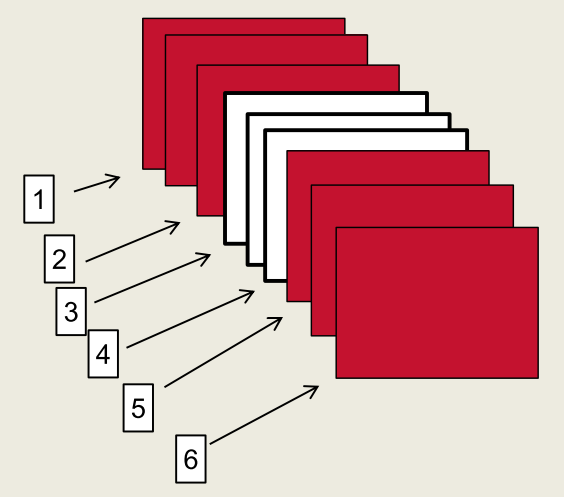
\includegraphics[width=0.4\textwidth]{eventos.png}
	\caption{\small Ejemplo de una secuencia de eventos. Los cuadros coloreados y blancos indican eventos con poca o mucha relevancia, respectivamente. Los marcadores indican transiciones entre fases de poco y mucho interés. Obtenido de \cite{Kelley2014}.}
	\label{img:sleep_eventos}
\end{figure}

%Ejemplo:
%At some location (cue), something big and orange (Tiger) moved from left to right resulting in pain (event)

Además, este diseño permite que el sistema cambie su opinión sobre un evento, mediante aprendizaje reforzado. Si se repiten eventos, pero la consecuencia deja de ser la misma, entonces el sistema se acostumbra.


\subsubsection{Aspectos fuera del alcance del proyecto}\label{sec:otros_aspectos}
%% =====================================================================

A continuación se presentan algunos estudios relacionados con aspectos de una memoria a largo plazo que escapan de los requerimientos para este proyecto o que simplemente no son basados en la taxonomía de la memoria humana. Estos trabajos sólo se presentan a modo de completitud, pues no permiten resolver el objetivo de este proyecto, sino que sólo comprender otros enfoques y acercamientos a la solución. 

El sistema propuesto por Ho et al. \cite{Ho2009} busca modelar la memoria de forma suficientemente general, como para permitir el traspaso de los recuerdos de un robot a otro, independientemente de que el hardware sea distinto; El costo de esto, es que se reduce la personalización de cada robot. Ho et al. además aplican la teoría \textit{Roboética}, sugerida por Veruggio y Operto \cite{Veruggio2006}, de donde derivan restricciones de diseño, relativas al manejo de información privada de los usuarios.

En \cite{KimMinJoo2016}, Kim et al. plantean el uso de Deep Learning para modelar la memoria episódica y la planificación de acciones de manera holística. En su implementación, los procesos de codificación, almacenado y recuperación de episodios son manejados como uno solo. Los procesos de decaimiento y relevancia son abstraídos, para ser manejados automáticamente por la red.

Thorsten et al. \cite{Spexard2008} proponen una memoria LTM para el robot BIRON. En su trabajo, se abstraen de la clasificación entre memorias episódica y semántica, pues todos los datos de largo plazo almacenados por el robot son considerados LTM. La memoria almacena sólo datos de alto nivel, obtenidos tras el procesamiento de streams de datos básicos, como cámaras, micrófonos o actuadores. Los datos almacenados corresponden a un historial de percepciones y acciones de alto nivel realizadas, como: detecciones de objetos, interacciones verbales o la descripción de movimientos realizados. A pesar de su simplicidad, esta arquitectura centralizada permite reducir las dependencias entre cada componente y el ancho de banda utilizado para retransmitir la información entre procesos.

La memoria de largo plazo procedural es estudiada por Salgado et al. \cite{Salgado2012}, donde demuestran que a través de ella se puede mejorar el desempeño del robot en tareas repetitivas. En 2014 Winkler et al. desarrollaron CRAMm \cite{Winkler2014}, un sistema para el manejo de memoria semántica y procedural basado en KnowRob \cite{Tenorth2013}, con el fin de dar soporte a las tareas de manipulación de su plataforma robótica. Mediante CRAMm, el robot puede tener conocimiento de los objetos del entorno, sus posiciones habituales y las rutinas de manipulación apropiadas para cada caso. Por ejemplo, puede saber que la leche es un objeto perecible, por lo que probablemente pueda ser encontrada en el refrigerador, más aún, CRAMm provee procedimientos para abrir ese contenedor y obtener el objeto.


%% =====================================================================

%% =====================================================================

%% =====================================================================

%% =====================================================================

%% =====================================================================

%% =====================================================================

%% =====================================================================

%% =====================================================================
%% =====================================================================
\section{Aspectos relevantes para el diseño}
%% =====================================================================
%% =====================================================================
%% =====================================================================

Esta sección presenta en detalle el marco teórico requerido para el diseño del software del proyecto. Se detallan aspectos de diseño para la memoria episódica y semántica. Además se revisan implementaciones de memoria emocional y relevancia histórica para modular el almacenamiento, deterioro y la adquisición de episodios. Los trabajos presentados acá fueron seleccionados a partir del estudio realizado en la Sección \ref{sec:revision_LTM}.

%% =====================================================================
%% =====================================================================
%% =====================================================================
\subsection{Memoria explícita}\label{sec:ltm_exp}
%% =====================================================================
%% =====================================================================
%% =====================================================================

La implementación de un sistema de memoria episódica no puede ser completamente separada de la memoria semántica. La primera almacena eventos y su contexto espacio-temporal, a la vez que la otra almacena información sobre cada entidad del episodio. Así, es posible recordar información de un objeto y su evolución histórica ligada a los eventos almacenados.

De acuerdo a lo estudiado en la Sección \ref{sec:revision_LTM}, no existe un consenso sobre los contenidos, el formato o las herramientas para implementar una memoria episódica. Sin embargo, si existe una aceptación generalizada sobre los requerimientos mínimos y deseables para su diseño \cite{Vijayakumar2014,Ho2009,Jockel2008}. Particularmente, Stachowicz en su trabajo del año 2012 \cite{Stachowicz2012} deriva un conjunto de 11 requisitos mínimos para la construcción de una memoria episódica, a partir de características cognitivas de sistemas episódicos naturales, extendidas con propiedades deseables desde un punto de vista técnico. Estos requisitos $(\mathcal{R}_{1},\ldots,\mathcal{R}_{11})$, descritos a continuación, permiten dar una base para el diseño del software del proyecto.


\subsubsection{Aspectos de diseño requeridos:}
%% =====================================================================


\begin{itemize}[topsep=0pt]
	\setlength\itemsep{0.2em}
	\item \RStachowicz{1} {\bfseries Contenido:}
	La información de eventos pasados debe ser recolectada e indexada respecto a su contexto espacio-temporal: Qué, dónde y cuándo pasó. El campo ``Qué'' debe permitir almacenar información variable, organizada en estructuras de datos que no se conocen de antemano y que se ajustan a diversos módulos de procesamiento. 
	
	\item \RStachowicz{2} {\bfseries Estructura:}
	Cada evento en conjunto con su contexto espacio-temporal forman una única representación integrada, que debe ser recolectada como un todo, en caso de recolectar cualquiera de las características del evento.
	
	\item \RStachowicz{3} {\bfseries Flexibilidad:}
	La información almacenada es declarativa por naturaleza, y puede ser flexiblemente almacenada. Particularmente, puede interactuar con conocimiento semántico, incluso si este fue obtenido con posterioridad a la codificación del episodio.
	
	\item \RStachowicz{4} {\bfseries Unicidad:}
	La memoria episódica cuenta con sólo una instancia de cada evento para su entrenamiento, pues cada evento tiene características específicas a la situación. Es decir, cada episodio es único y no puede ser generalizado o entrenado a partir de una secuencia de episodios.
	
	\item \RStachowicz{5} {\bfseries Introspección:}
	Recuerdos episódicos pueden ser almacenados por periodos de segundos, minutos, días o años. Es posible hablar sobre eventos asociados y acceder a ellos para introspección.
	
	\item \RStachowicz{6} {\bfseries Perspectiva:}
	La memoria episódica debe lidiar con datos específicos al evento, lo que implica una perspectiva. Es decir, eventos recordados deben mantener la misma perspectiva que se tenía en la experiencia original \cite{CLAYTON20092330}. Por otro lado, la memoria semántica generalmente se puede abstraer de la perspectiva y aspectos situacionales.
	
	\item \RStachowicz{7} {\bfseries Anidamiento:}
	Los eventos almacenados en la memoria episódica pueden variar en tiempo y extensión. Particularmente, pueden ocurrir eventos dentro del lapso temporal de otro, ambos asociados al mismo contexto episódico.
	
	\item \RStachowicz{8} {\bfseries Transposición:}
	Los eventos almacenados en la memoria episódica pueden variar en tiempo y extensión. Particularmente, un evento A puede iniciar antes B, pero terminar durante la vida de B.
	
\end{itemize}

\subsubsection{Aspectos de diseño deseables:}
%% =====================================================================

\begin{itemize}[topsep=0pt]
	\setlength\itemsep{0.2em}
	\item \RStachowicz{9} {\bfseries No intrusivo:}
	Se espera que la LTM no requiera dependencias de módulos externos para poder funcionar y representar los datos. A la vez, no puede depender en que los otros módulos no cambien la representación de sus datos.
	
	\item \RStachowicz{10} {\bfseries Eficiente:}
	El sistema debe ser lo suficientemente eficiente para tolerar el manejo de una alta tasa de eventos, sin degradar el funcionamiento del robot. Es decir, todos los eventos deben ser procesados eventualmente, aún cuando el robot esté ocupando gran parte de sus recursos, y sin generar hambruna de CPU ni de ancho de banda (de disco y red) al resto de los procesos.
	
	\item \RStachowicz{11} {\bfseries Escalable:}
	Los costos asociados al manejo de la información (agregar, eliminar, actualizar y buscar datos) en la memoria deben escalar bien, respecto a la cantidad de datos almacenados. La memoria debe mantener los costos acotados, dentro de un rango que no entorpezca su uso.
	
\end{itemize}


%% =====================================================================
%% =====================================================================
%% =====================================================================
\subsection{Modulación de procesos cognitivos}\label{sec:theory-modulation}
%% =====================================================================
%% =====================================================================
%% =====================================================================

El almacenamiento, deterioro y recolección de episodios puede ser afectado por diversos factores. A continuación se detallan estudios que influencian el diseño, en cuanto a la modulación de tales procesos cognitivos, a partir de la memoria emocional y la relevancia histórica de los episodios.


\subsubsection{Memoria emocional}
%% =====================================================================
% Para más refs sobre emociones ver Deutsch2008

% uso de memoria emocional
La importancia de un evento se ve fuertemente influenciada por el estado emocional de una persona, o en este caso, el robot. Así, se puede dar prioridad a unos eventos por sobre otros, afectando los procesos cognitivos. Particularmente, un evento importante emocionalmente podría ser más fácilmente recordado, o ser almacenado por un periodo más largo \cite{Deutsch2008}.

La implementación de la memoria emocional requiere como mínimo de un mapeo entre los estímulos percibidos por el robot y las sensaciones emocionales que estos generan. Dood et al. \cite{Dodd2005} propone el uso de la teoría emocional de reacciones de Haikonen, que considera a una emoción como una combinación de estímulos básicos. Las sensaciones elementales son: bienestar, malestar, dolor, placer e interés.

Dood et al. proponen implementar las sensaciones a partir de distintos estímulos medidos en un robot:
\begin{itemize}
	\item Actuador que se aproxima a sus límites de movimiento físico o de fuerza. 
	\item Nivel de iluminación percibido.
	\item Nivel de ruido acústico percibido.
	\item Ausencia o presencia de humanos. Falta de interacción.
	\item Cumplimiento de objetivos.
	\item Cumplimiento de expectativas.
\end{itemize}

Sistemas más avanzados, incluso pueden considerar la generación de reacciones emocionales, basándose en las sensaciones derivadas anteriormente. En la Figura \ref{img:emotional_haikonen} se muestran las reacciones generadas según el modelo de Haikonen. Además, estas se podrían reflejar en la personalidad del robot, por ejemplo, mediante gestos, vocabulario o nivel de aceptación para realizar una acción. Kasap et al. \cite{Kasap2010} utilizan un sistema llamado \textit{Emotion Engine}, para generar reacciones emocionales y simular cambios de personalidad de un robot, según las sensaciones percibidas.

\begin{figure}[!ht]
	\centering
	\begin{tabular}{| l | l |}
		\hline
		\rowcolor{gray!50}
		Sensación Elemental & Reacción  \\ 
		\hline Bueno: gusto, aroma & Aceptación, Acercar \\ 
		\hline Malo: gusto, aroma & Rechazo, Alejar \\ 
		\hline Dolor: autoinfligido  & Alejar, Desistir \\ 
		\hline Dolor: agente externo & Agresión \\ 
		\hline Dolor: sobre esfuerzo & Sumisión \\ 
		\hline Placer & Mantener, Acercar \\ 
		\hline Acierto & Mantener atención \\ 
		\hline Desacierto & Migrar atención \\ 
		\hline Novedad & Enfocar atención \\ 
		\hline 
	\end{tabular} 
	\caption{\small Sensaciones elementales y sus reacciones correspondientes, según el modelo de Haikonen. Obtenido de \cite{Dodd2005}.}
	\label{img:emotional_haikonen}
\end{figure}

Para su uso efectivo dentro de un esquema LTM, se espera que las sensaciones reportadas incluyan un nivel de intensidad. Según el nivel percibido en cada episodio, es posible clasificarlos entre eventos muy o poco relevantes. Los más relevantes tendrán mayor probabilidad de ser recuperados al recordar. Deutsch et al.  \cite{Deutsch2008} consideran que la intensidad de las sensaciones es importante, pues permite evitar costos de búsqueda lineales dentro de todos los episodios almacenados.

En el año 1980 Plutchik presenta la Rueda de las Emociones \cite{plutchik1980}, que se muestra en la Figura \ref{img:plutchik}. Su trabajo es uno de los más influyentes para la clasificación de las emociones y sus respuestas. Plutchik propone 8 emociones primarias, cada una de carácter bipolar: ira - miedo, alegría - tristeza, confianza - aversión, sorpresa - anticipación. De manera similar a los colores, cada emoción tiene un nivel de intensidad asociado, y puede ser mezclada con otra para formar distintas emociones. La rueda además muestra 8 emociones avanzadas de carácter bipolar, formadas a partir de las 2 emociones primarias adyacentes.

\begin{figure}[!ht]
	\centering
	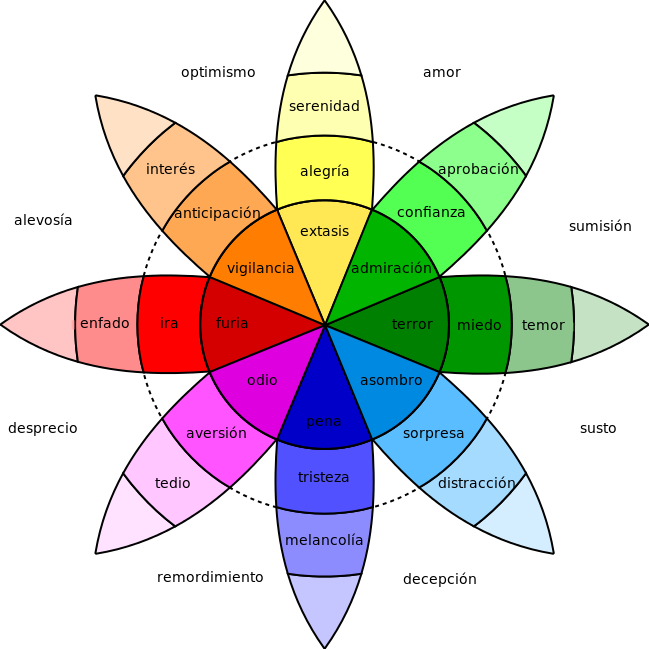
\includegraphics[width=0.7\textwidth]{plutchik-wheel.png}
	\caption{\small Rueda de las Emociones de Plutchik. Propone 8 emociones primarias de carácter bipolar y 3 niveles de intensidad. Cada emoción compleja se componen de sus 2 emociones primarias adyacentes.}
	\label{img:plutchik}
\end{figure}


\subsubsection{Relevancia histórica}
%% =====================================================================
% - Sobre concepto de relevancia historica
% - mezlcla y relevancia generalizada
% - algoritmo y graph
Este concepto es una representación del olvido o pérdida de interés en las memorias episódicas en el caso robótico. Está directamente relacionado a la edad de un episodio, a menor antigüedad, mayor es su importancia, lo que se traduce en una mayor probabilidad de recordar ese episodio.

La implementación de relevancia histórica es estudiada por Dood et al. \cite{Dodd2005}, donde presenta una estrategia para su implementación y su interacción con la memoria emocional. Propone el uso de un indicador de relevancia generalizado, obtenido al combinar la intensidad de los dos indicadores. Y además, propone un modelamiento matemático para representar el decaimiento de la relevancia histórica en el tiempo.

\todounsure{Es necesario poner ecuaciones y curvas de decaimiento??}
